\chapter{Applications}
In this section, we describes how to use WEC-Sim to model two different WECs.  The first application models a two-body point absorber WEC and the second application models an OSWEC. 
%%%%%%%%%%%%%%%%%%%%%%%%%%%%%%%%%%%%%%%%%%%%%%%%%%%%%%%%%%
\section{Reference Model 3 Two-Body Point Absorber}
%%%%%%%%%%%%%%%%%%%%%%%%%%%%%%%%%%%%%%%%%%%%%%%%%%%%%%%%%%
\subsection{Geometry Definition}
As the first application of the WEC-Sim code, We selected the Reference Model 3 (RM3) two-body point absorber design. Although the WEC is free to move in all 6DOF in response to wave motion, power is captured in the relative heave direction. The RM3 device was selectedonly  because the design has already been well characterized both numerically and experimentally as a result of the DOE-funded Reference Model Project, more information on this project available at \href{http://energy.sandia.gov/rmp}{http://energy.sandia.gov/rmp}. In addition, the device has relatively simple operating principles and is representative of what WEC industry is currently pursuing. RM3 is a simple two-body point absorber, consisting of a float and a reaction plate. The full-scale dimensions of the RM3 are shown in Figure \ref{RM3_Geom}, and the mass properties are defined in Table \ref{RM3_MassProps}.  

        \begin{figure}[H]
        \centering
        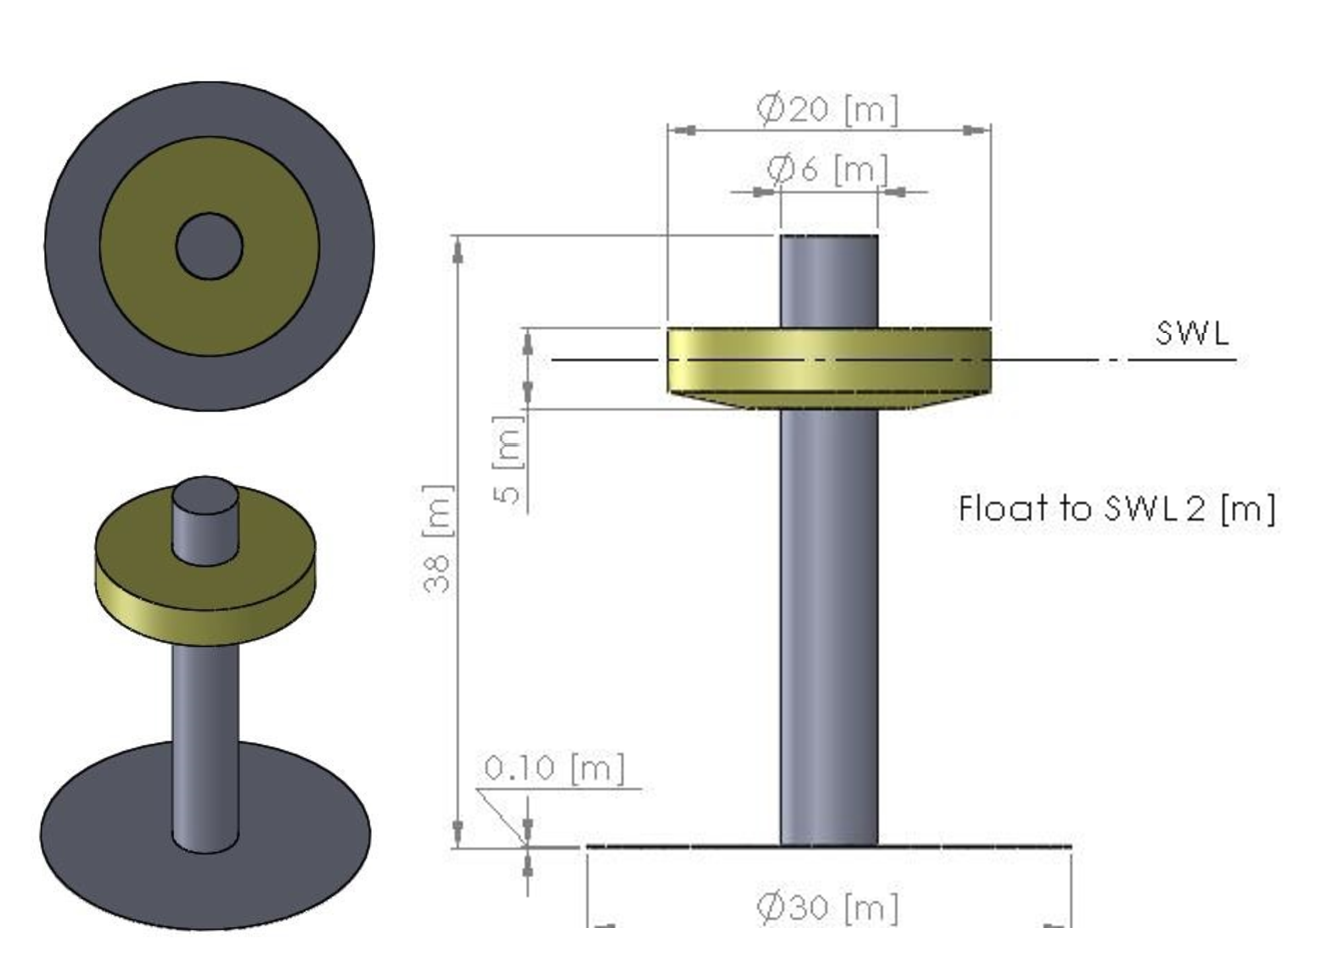
\includegraphics[width=0.7\textwidth]{application/images/RM3_Geom}
        \caption{RM3 heaving two-body point absorber full-scale dimensions}
        \label{RM3_Geom}
        \end{figure}

        \begin{table}[H]
        \centering
        \caption{RM3 heaving two-body point absorber full-scale mass properties}
        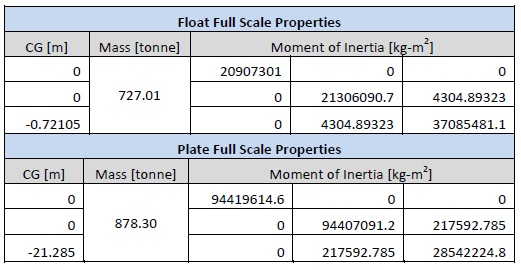
\includegraphics[width=0.8\textwidth]{application/images/RM3_MassProps}
        \label{RM3_MassProps}
        \end{table}

%%%%%%%%%%%%%%%%%%%%%%%%%%%%%%%%%%%%%%%%%%%%%%%%%%%%%%%%%%
\subsection{Modeling RM3 in WEC-Sim}
In this section,  we provide a step by step tutorial on how to set up and run the RM3 simulation in WEC-Sim. We have also created a supplemental RM3 WEC-Sim Tutorial Video to demonstrate how to set up and run the RM3 simulation in WEC-Sim. The tutorial video is included in the WEC-Sim code download package under the documentation folder. 

As described in \hyperlink{chapter.3}{Chapter 3}, all WEC-Sim models consist of a input file (\texttt{wecSimInputFile.m}), and a Simulink model file (\texttt{RM3.slx}). To run the WEC-Sim simulation, the user needs to provide results from the WAMIT, frequency-domain BEM solver, to populate the WEC-Sim hydrodynamic coefficients. The WAMIT hydrodynamic results were pregenerated. The WAMIT output file corresponds to the \texttt{buoywamit.out} file, contained in the wamit subfolder. Note that all the hydrodynamic coefficients MUST be output at the center of gravity. In addition, the user needs to specify the 3-D geometry file in the form of a \texttt{<STL file name>.stl} file with the origin of the coordinate system at the center of gravity for the WEC-Sim visualizations. For the RM3 run consisting of a buoy and a spar plate, these files correspond to the \texttt{float.stl} and \texttt{plate.stl} files, respectively, which are located in the geometry subfolder.\\

%%%%%%%%%%%%%%%%%%%%%%%%%%%%%%%%%%%%%%%%%%%%%%%%%%%%%%%%%%
\textbf{\textit{RM3 Simulink Model File}}\\
The first step to initiate a WEC-Sim simulation is to create the Simulink model file by dragging and dropping blocks from the WEC-Sim library into the \texttt{<WEC model name>.slx} file (see \hyperlink{chapter.4}{Chapter 4} for more details). 

\textbf{Step 1:} Place two \texttt{Rigid Body} blocks from the WEC-Sim library in the Simulink model file, one for each RM3 rigid body, as shown in Figure \ref{RM3_WECSim_Body2}. 

\textbf{Step 2:} Double click on the \texttt{Rigid Body} block, and rename the instances of the body. The first body should be titled \texttt{body(1)}, and the second body should be titled \texttt{body(2)}. Additional properties of these body blocks are defined in the following RM3 MATLAB Input File section (Section~\ref{InputFile}). 

        \begin{figure}[H]
        \centering
        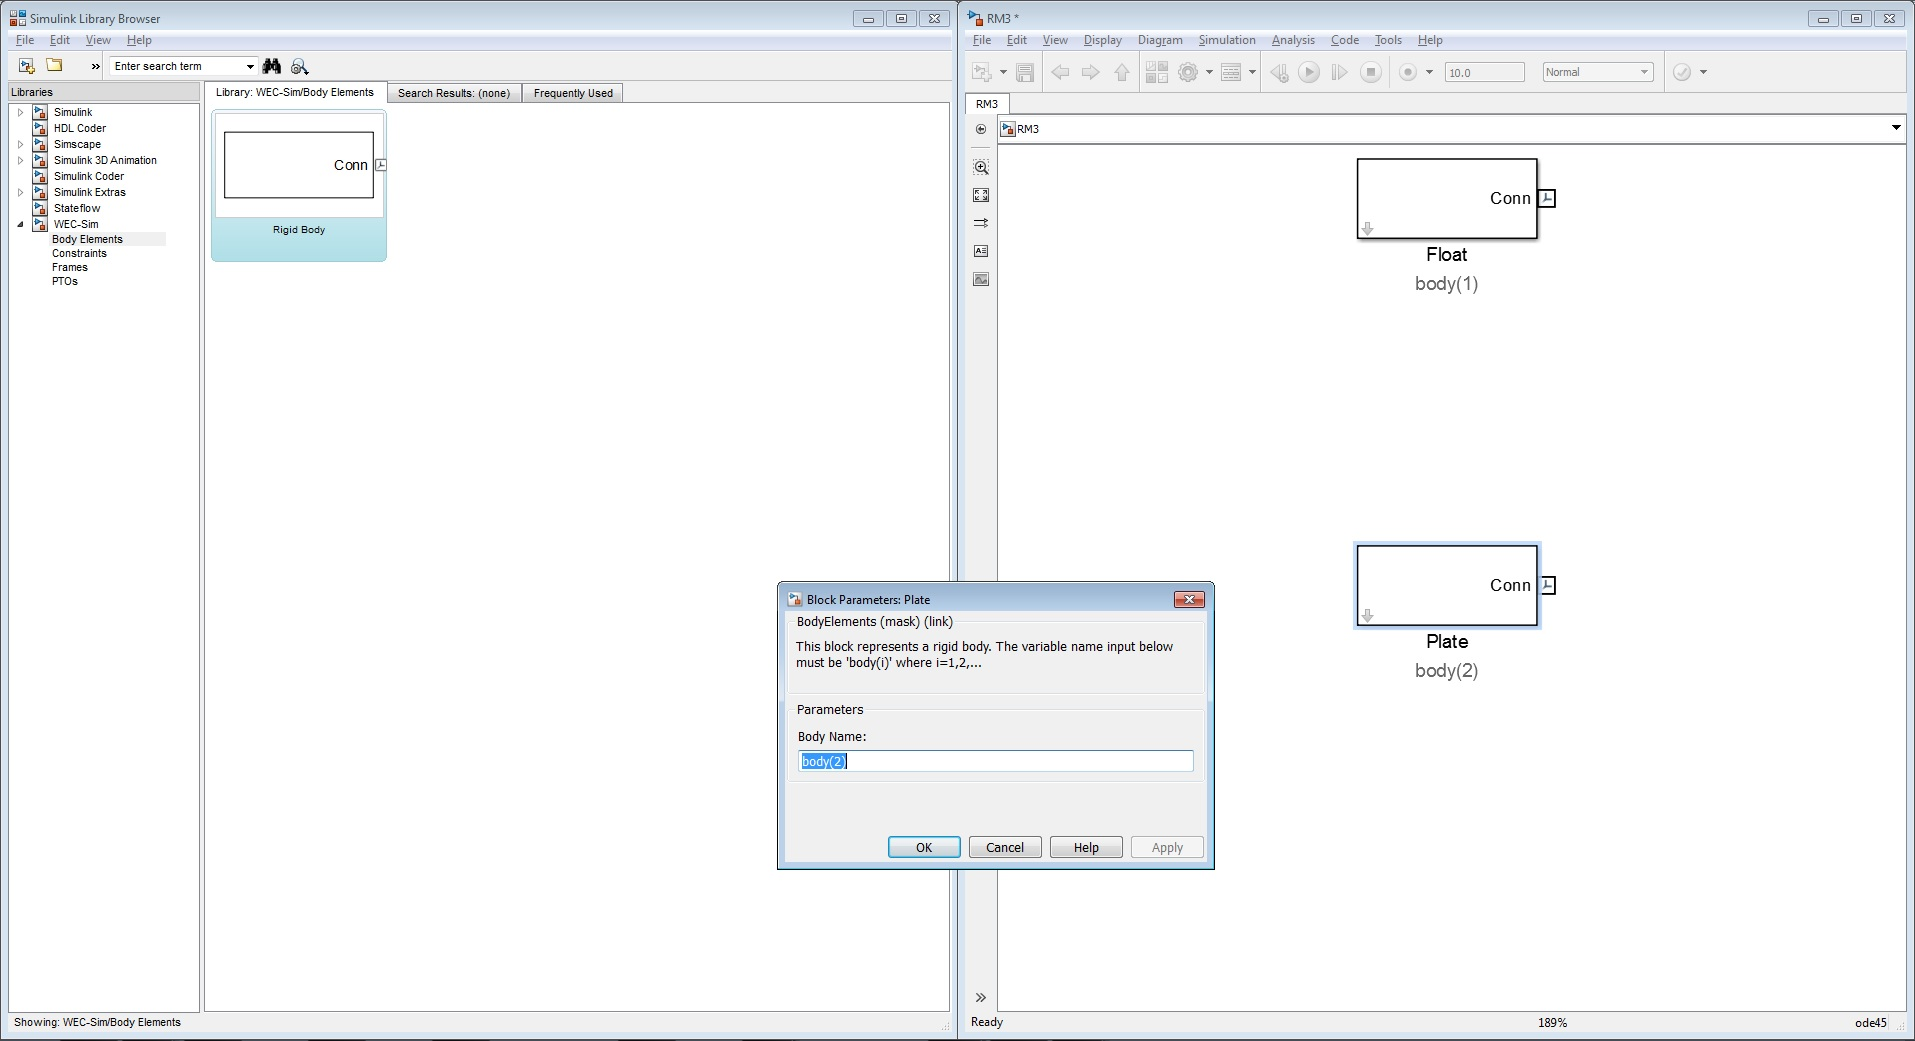
\includegraphics[width=0.9\textwidth]{application/images/RM3_WECSim_Body}
        \caption{Adding two \texttt{Rigid Body} blocks to the RM3 WEC-Sim model}
        \label{RM3_WECSim_Body2}
        \end{figure}

\textbf{Step 3:} Place the \texttt{Global Reference Frame} from the WEC-Sim library in the Simulink model file, as shown in Figure \ref{RM3_WECSim_SeaFloor}. The global reference frame acts as the seabed to which all other bodies are linked through joints or constraints.

        \begin{figure}[H]
        \centering
        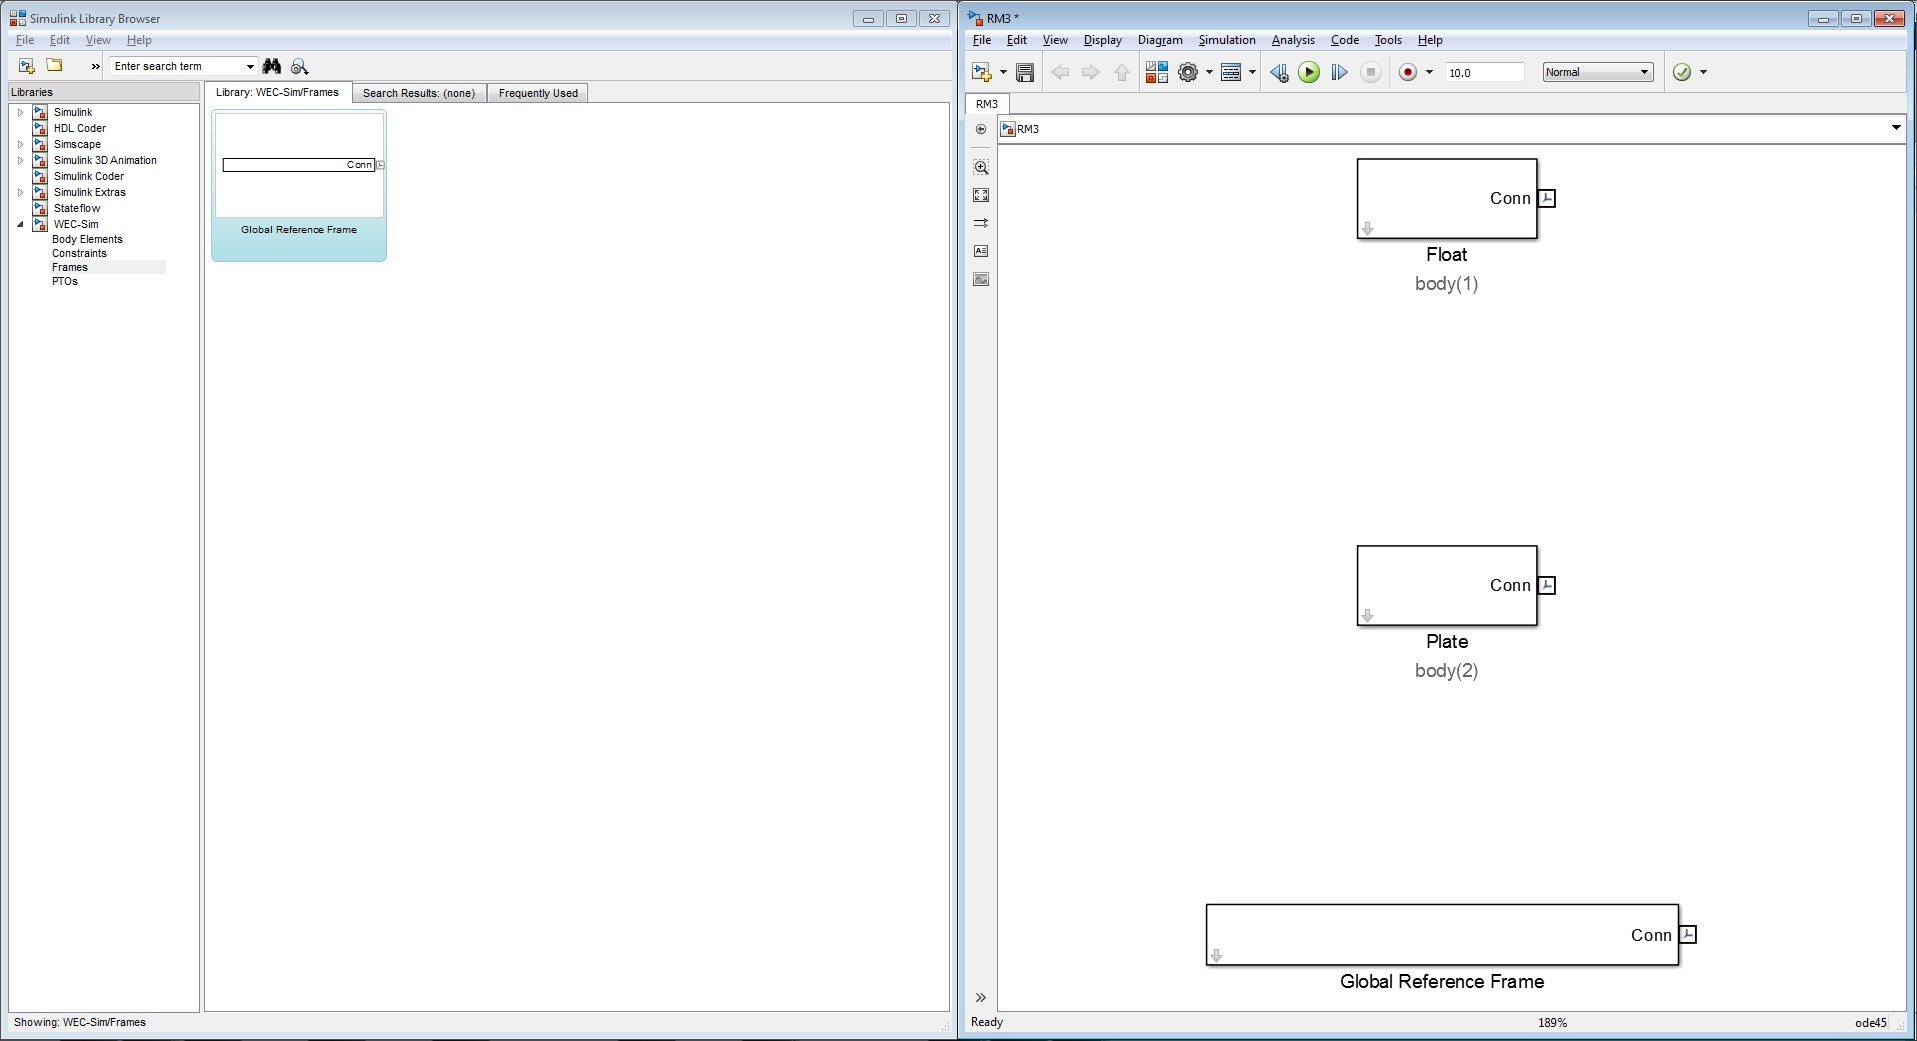
\includegraphics[width=0.9\textwidth]{application/images/RM3_WECSim_GlobalRef}
        \caption{Adding the \texttt{Global Reference Frame} block to the RM3 WEC-Sim model}
        \label{RM3_WECSim_SeaFloor}
        \end{figure}

\textbf{Step 4:} Use the \texttt{Floating} constraint block to connect the plate to the seabed. This is done because the RM3 is free to move in all 6 DOF relative to the global reference frame. Step 4 and 5 connections are shown in Figure \ref{RM3_WECSim}. 

        \begin{figure}[H]
        \centering
        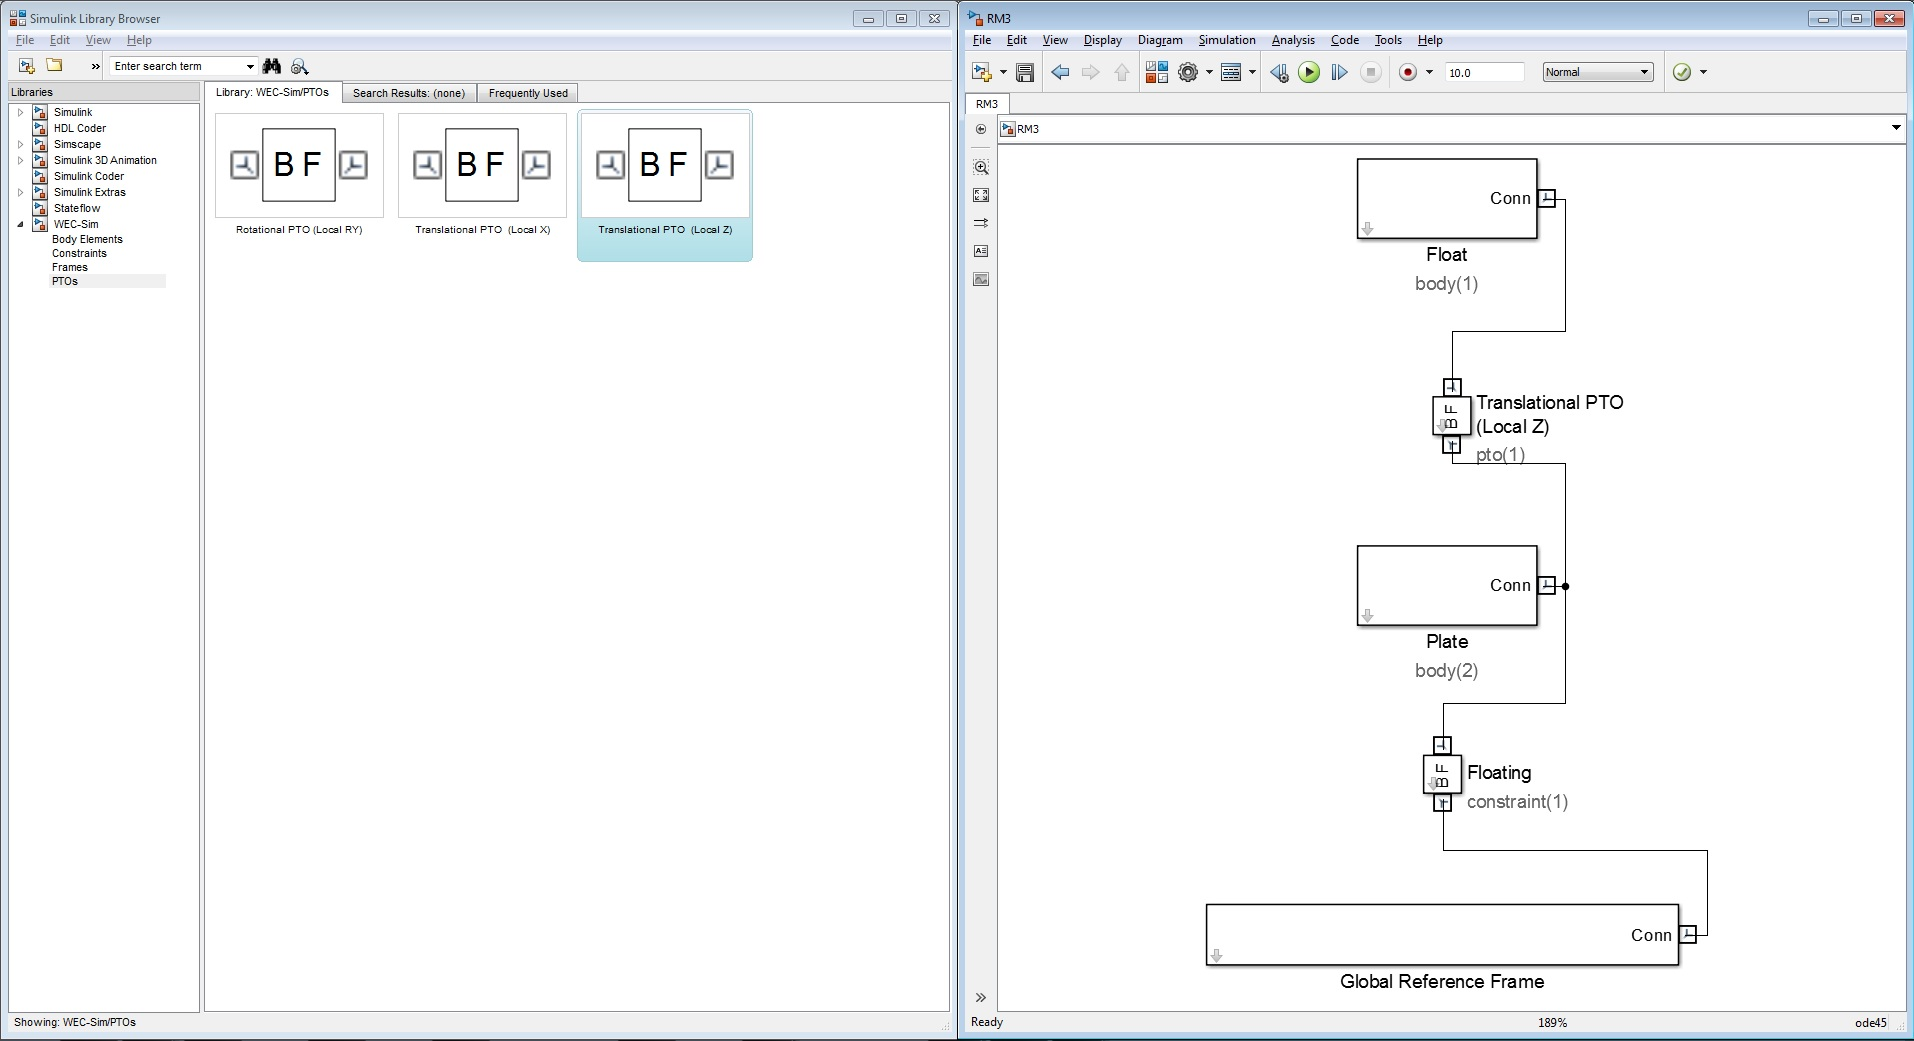
\includegraphics[width=0.9\textwidth]{application/images/RM3_WECSim}
        \caption{Adding the pto and constraint blocks to the RM3 WEC-Sim Simulink model}
        \label{RM3_WECSim}
        \end{figure}

\textbf{Step 5:} Place a \texttt{Translational PTO (Local Z)} PTO block to connect the float to the spar. This is necessary because the float is restricted to heave motion relative to the plate. For the RM3 simulation, the translational PTO block is used to model the WEC's PTO as a linear damper. The parameters are defined in the RM3 MATLAB Input File section (Section~\ref{InputFile}). \\

When setting up a WEC-Sim model, it is important to note the base and follower frames. For example, for the constraint between the plate and the seabed, the seabed should be defined as the base because it is the Global Reference Frame.  Similarly, for the PTO between the float and the plate, the plate should be defined as the base.\\

%%%%%%%%%%%%%%%%%%%%%%%%%%%%%%%%%%%%%%%%%%%%%%%%%%%%%%%%%%
\textbf{\textit{RM3 MATLAB Input File}}\label{InputFile}\\
In this section, we define the WEC-Sim MATLAB input file for the RM3 model. Each of the lines are commented to explain the purpose of the defined parameters. For the RM3 model, the user must define the simulation parameters, body properties, PTO, and constraint definitions. The specified input parameters for RM3 are shown in Figure \ref{fig:RM3inputFile}. \\

\begin{figure}[H]
\centering
\lstinputlisting{application/images/RM3wecSimInputFile.m}
\caption{WEC-Sim input file for the RM3 point absorber).}
\label{fig:RM3inputFile}
\end{figure}

%%%%%%%%%%%%%%%%%%%%%%%%%%%%%%%%%%%%%%%%%%%%%%%%%%%%%%%%%%
\textbf{\textit{RM3 WEC-Sim Model}}\\
Once the WEC-Sim Simulink model is set up and the RM3 properties are defined in the MATLAB input file, the user can then run the RM3 model in WEC-Sim.  Figure \ref{RM3_WECSim_GUI} shows the final RM3 Simulink model and the WEC-Sim GUI during the simulation. For more information on using WEC-Sim to model the RM3 device, refer to \cite{kelley_ruehl_preliminary_2014} and \cite{y._yu_development_2014}.

        \begin{figure}[H]
        \centering
        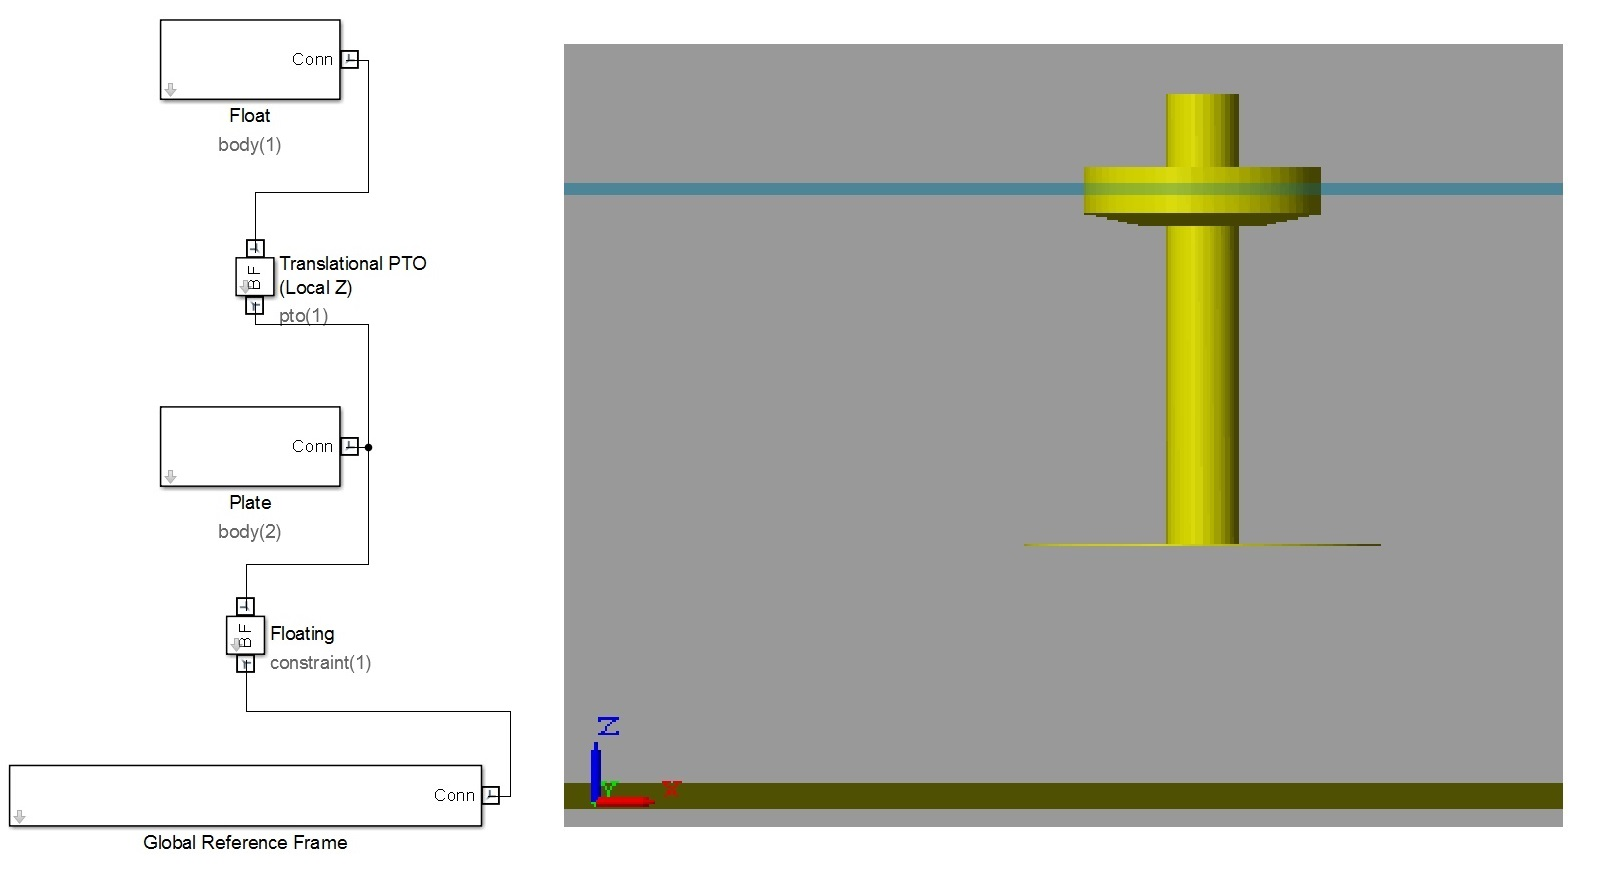
\includegraphics[width=1\textwidth]{application/images/RM3_WECSim_GUI}
        \caption{RM3 modeled in WEC-Sim (left-hand side)  and with the GUI (right hand side)}
        \label{RM3_WECSim_GUI}
        \end{figure}

%%%%%%%%%%%%%%%%%%%%%%%%%%%%%%%%%%%%%%%%%%%%%%%%%%%%%%%%%%
\section{Oscillating Surge-Pitch Device}
%%%%%%%%%%%%%%%%%%%%%%%%%%%%%%%%%%%%%%%%%%%%%%%%%%%%%%%%%%
\subsection{Geometry Definition}
As the second application of the WEC-Sim code, the oscillating surge WEC (OSWEC) device. We selected the OSWEC because its design is fundamentally different from the RM3. This is critical because WECs span an extensive design space, and it is important to model devices in WEC-Sim that operate under different principles.  The OSWEC is fixed to the ground and has a flap that is connected through a hinge to the base that restricts the flap to pitch about the hinge. The full-scale dimensions of the OSWEC are shown in Figure \ref{OSWEC_Geom}, and the mass properties are defined in Table \ref{OSWEC_MassProps}.

%%%%%%%%%%%%%%%%%%%%%%%%%%%%%%%%%%%%%%%%%%%%%%%%%%%%%%%%%%
\subsection{Modeling OSWEC in WEC-Sim}
In this section, we provide a step by step tutorial on how to set up and run the OSWEC simulation in WEC-Sim. 

As described in \hyperlink{chapter.3}{Chapter 3}, all WEC-Sim models consist of a input file (\texttt{wecSimInputFile.m}), and a Simulink model file (\texttt{OSWEC.slx}). The WAMIT hydrodynamic results were also pregenerated. The WAMIT output file corresponds to the \texttt{oswec.out} file, contained in the wamit subfolder. In addition, the user needs to specify the 3-D geometry file in the form of a \texttt{<WEC model name>.stl} file about the center of gravity for the WEC-Sim visualizations. For the OSWEC run consisting of a flap and a base, these files correspond to the \texttt{flap.stl} and \texttt{base.stl} files, respectively, which are located in the geometry subfolder.

        \begin{figure}[H]
        \centering
        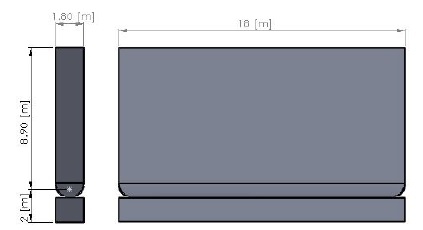
\includegraphics[width=0.8\textwidth]{application/images/OSWEC_Geom}
        \caption{OSWEC pitching device full-scale dimensions}
        \label{OSWEC_Geom}
        \end{figure}

        \begin{table}[H]
        \centering
        \caption{OSWEC pitching device full-scale mass properties}
        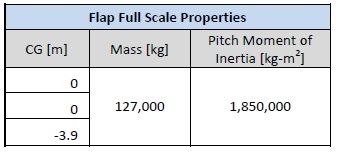
\includegraphics[width=0.6\textwidth]{application/images/OSWEC_MassProps}
        \label{OSWEC_MassProps}
        \end{table}
        
%%%%%%%%%%%%%%%%%%%%%%%%%%%%%%%%%%%%%%%%%%%%%%%%%%%%%%%%%%
\textbf{\textit{OSWEC Simulink Model File}}\\
The first step to set up a WEC-Sim simulation is to populate the Simulink model file by dragging and dropping blocks from the WEC-Sim library into the \texttt{<WEC model name>.slx} file, see \hyperlink{chapter.4}{Chapter 4}. 

\textbf{Step 1:} Place two \texttt{Rigid Body} blocks from the WEC-Sim library in the Simulink model file, one for each OSWEC rigid body, as shown in Figure \ref{OSWEC_WECSim_Body2}. 

        \begin{figure}[H]
        \centering
        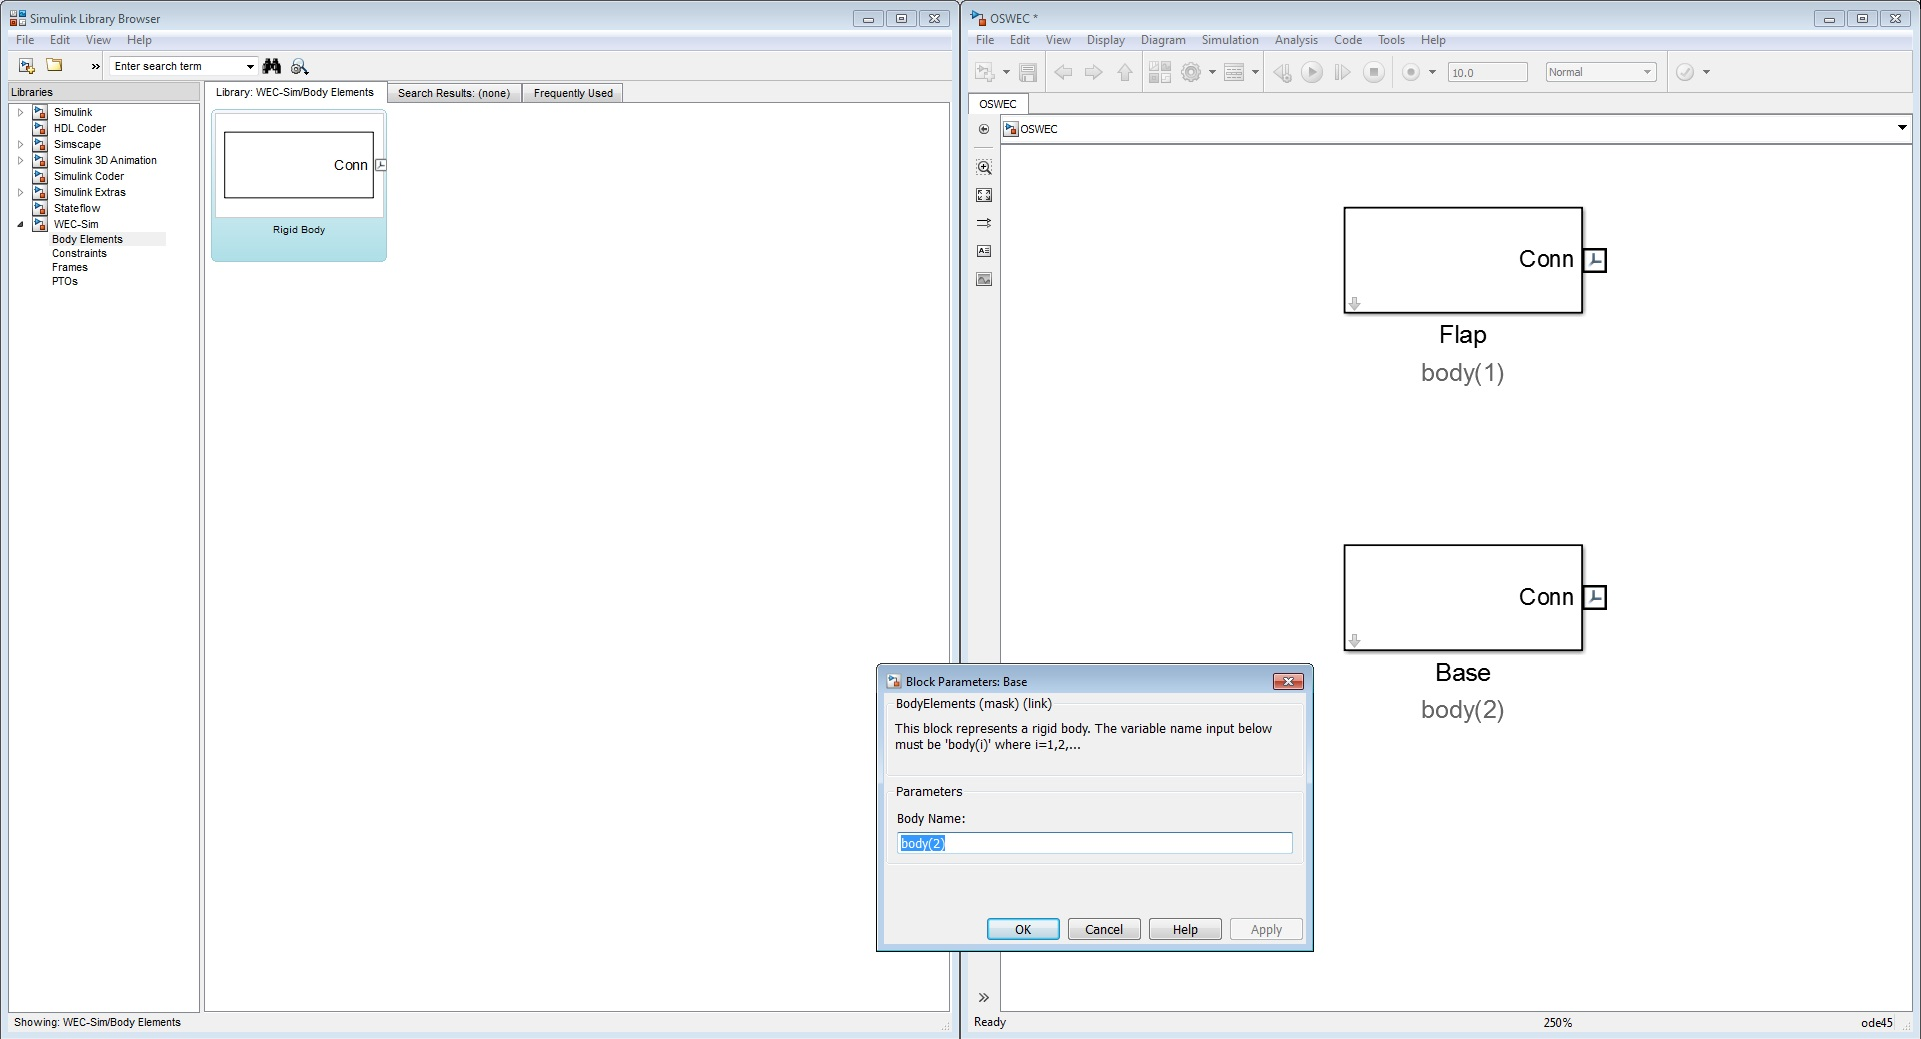
\includegraphics[width=0.9\textwidth]{application/images/OSWEC_WECSim_Body}
        \caption{Adding two \texttt{Rigid body} blocks to the OSWEC WEC-Sim model}
        \label{OSWEC_WECSim_Body2}
        \end{figure}

\textbf{Step 2:} Double click on the body block, and rename the instances of the body. The first body should be titled body(1), and the second body should be titled body(2). Additional properties of these body blocks are defined in the OSWEC MATLAB Input File section (Section~\ref{oswecInputFile}).

\textbf{Step 3:} Place the \texttt{Global Reference} block from the WEC-Sim library in the Simulink model file, as shown in Figure \ref{OSWEC_WECSim_SeaFloor}. The global reference frame acts as the base to which all other bodies are linked through joints or constraints.

        \begin{figure}[H]
        \centering
        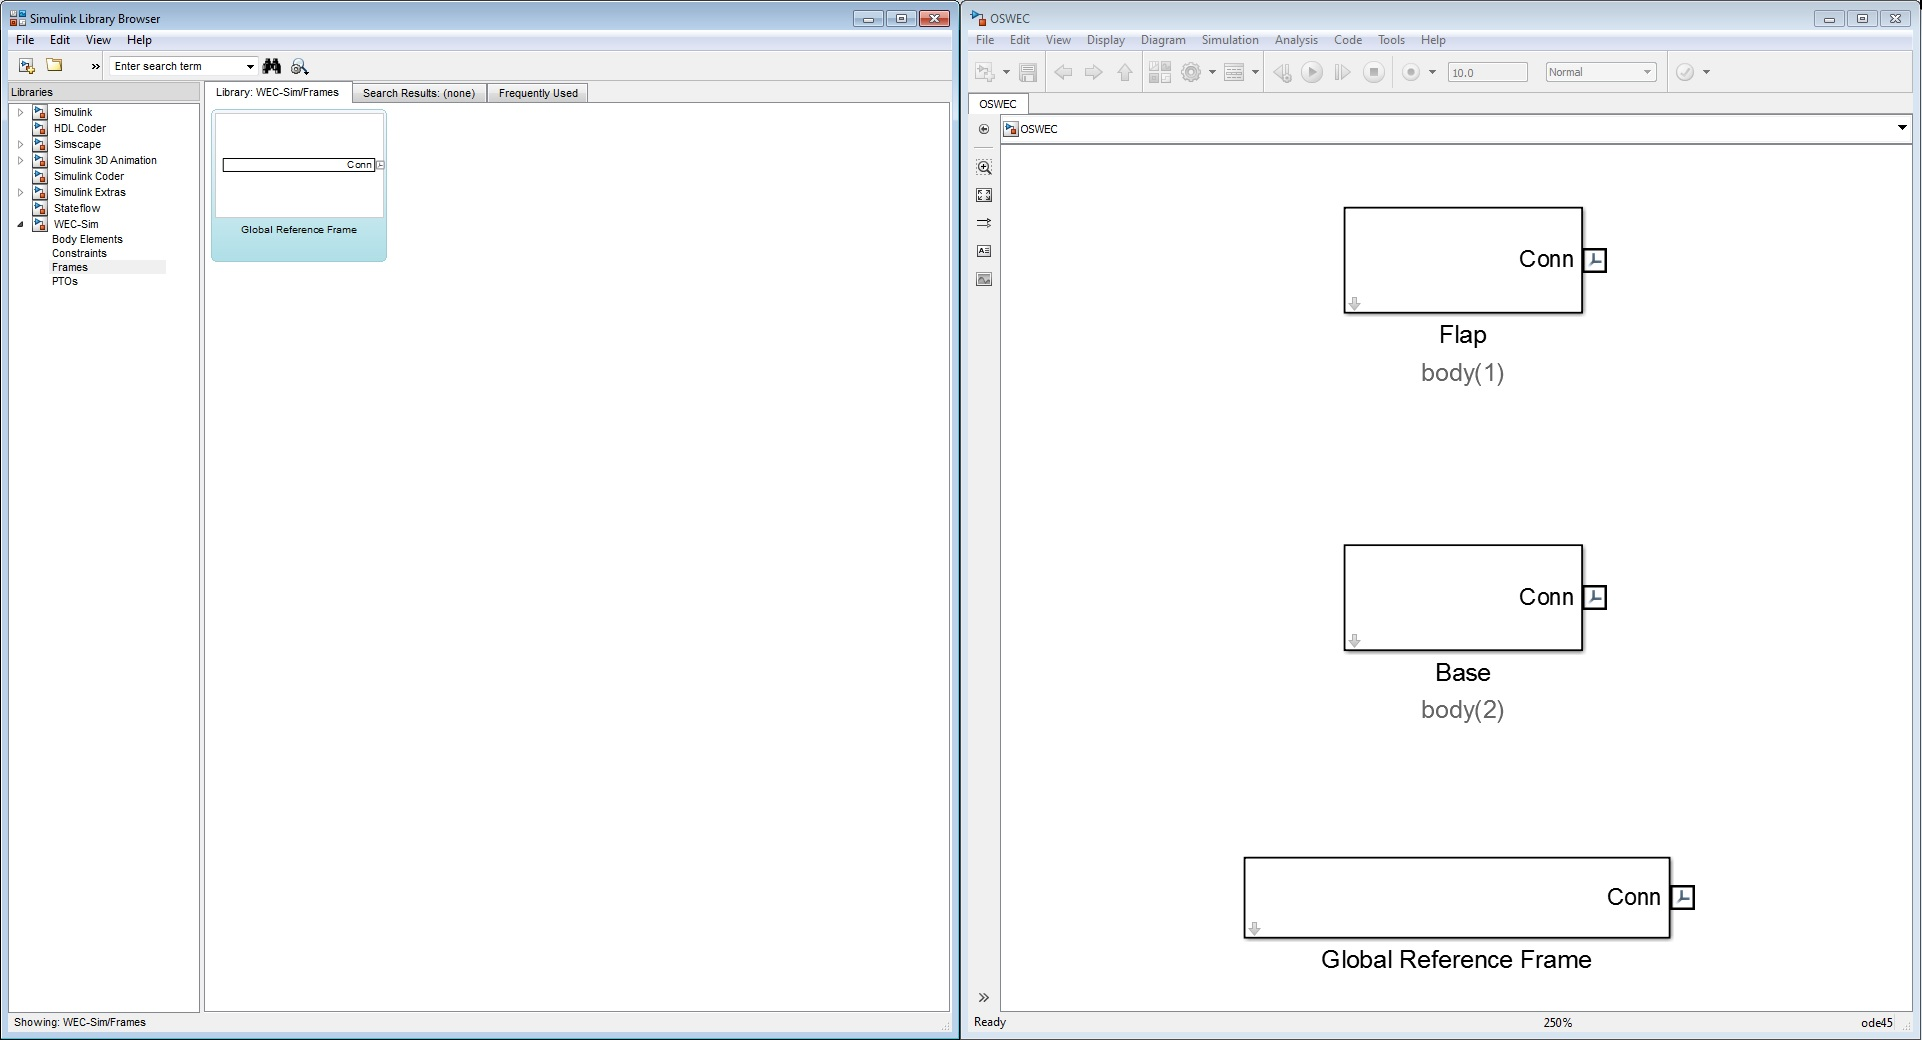
\includegraphics[width=0.9\textwidth]{application/images/OSWEC_WECSim_GlobalRef}
        \caption{Adding  a \texttt{Global Reference Frame} block to the OSWEC WEC-Sim model}
        \label{OSWEC_WECSim_SeaFloor}
        \end{figure}

\textbf{Step 4:} Place a \texttt{fixed} constraint block to connect the base to the seafloor. This is done because the OSWEC base is fixed relative to the global reference frame. Step 4 and 5 connections are shown in Figure \ref{OSWEC_WECSim}. 

        \begin{figure}[H]
        \centering
        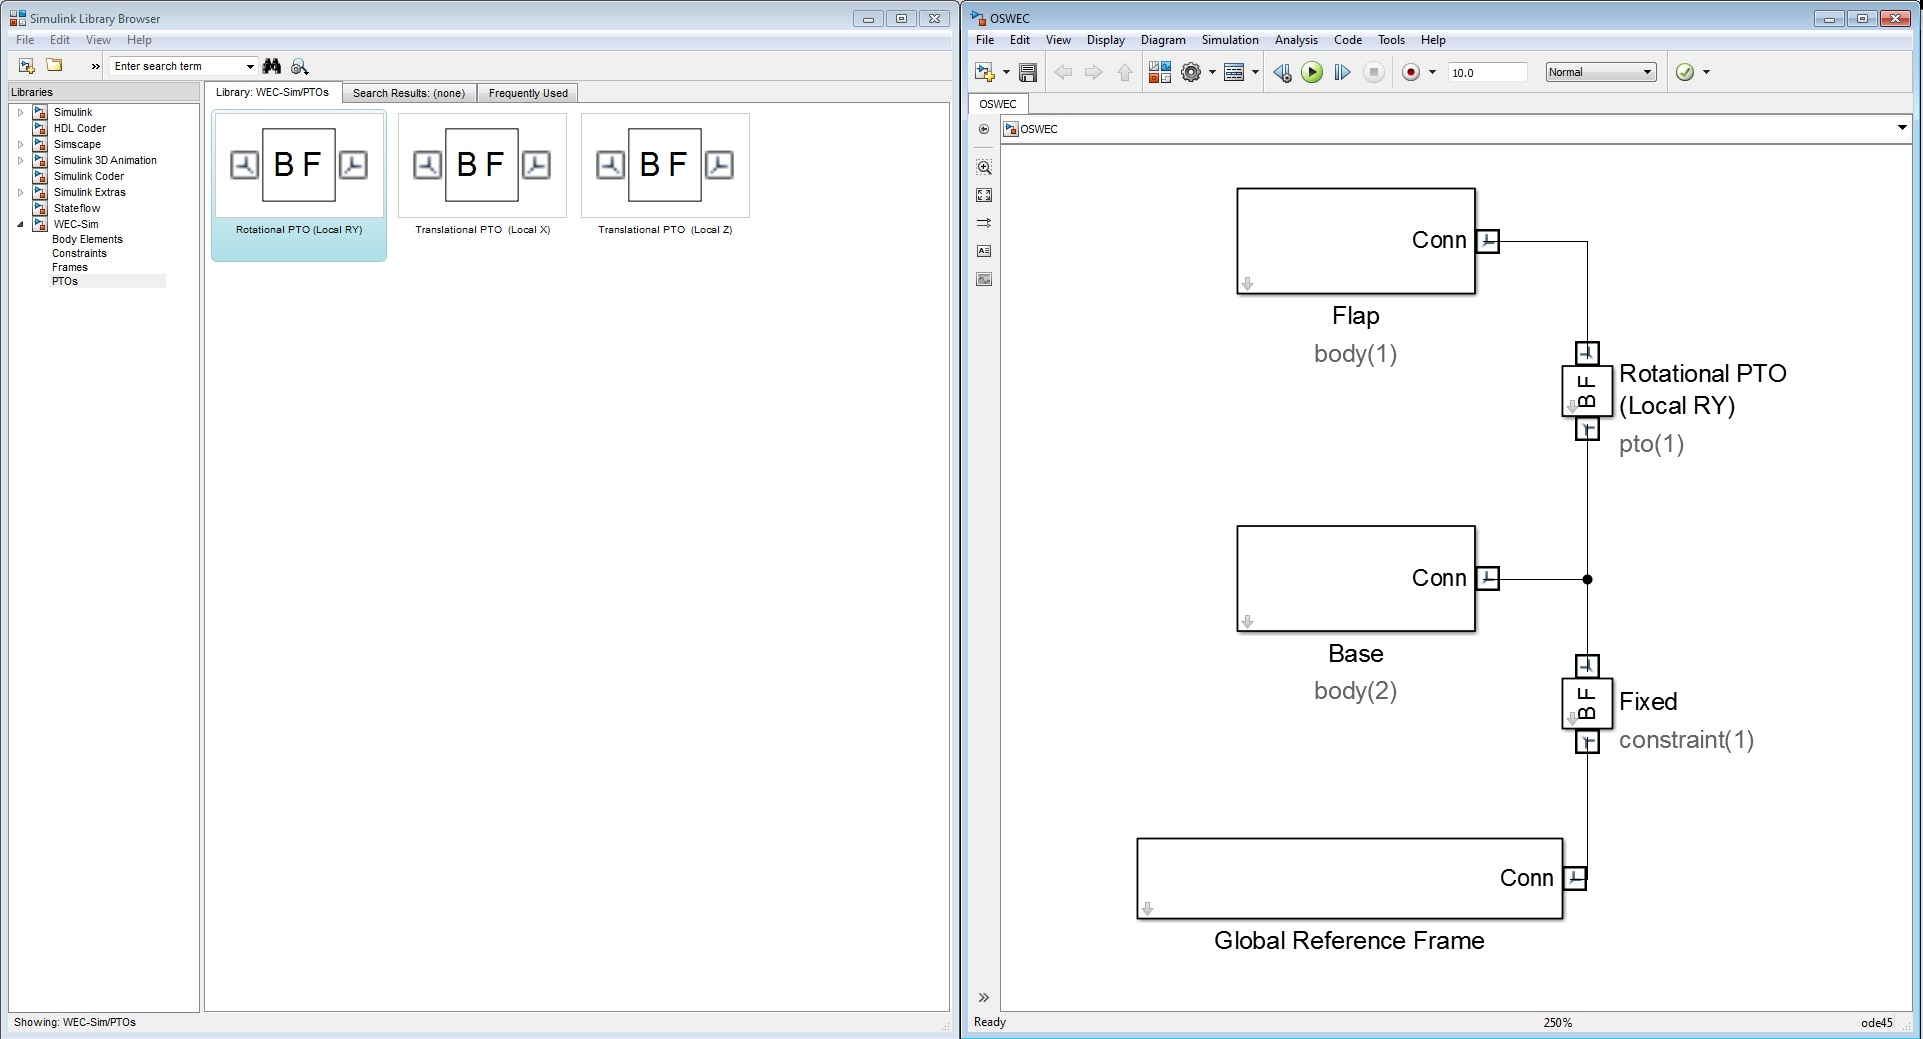
\includegraphics[width=0.99\textwidth]{application/images/OSWEC_WECSim}
        \caption{Adding pto and constraint blocks to the OSWEC WEC-Sim Simulink model}
        \label{OSWEC_WECSim}
        \end{figure}

\textbf{Step 5:} Place a \texttt{rotational PTO} block to connect the base to the flap. This is done because the flap is restricted to pitch motion relative to the base.  For the OSWEC simulation, the rotational PTO is used to model the WEC's PTO as a linear rotary damper. The input parameters are defined in the OSWEC MATLAB Input File section (Section~\ref{oswecInputFile}). \\

When setting up a WEC-Sim model, it is important to note the base and follower frames. For example, for the constraint between the base and the seabed, the seabed should be defined as the base because it is the Global Reference Frame.\\

%%%%%%%%%%%%%%%%%%%%%%%%%%%%%%%%%%%%%%%%%%%%%%%%%%%%%%%%%%
\textbf{\textit{OSWEC MATLAB Input File}} \label{oswecInputFile}\\
In this section, the WEC-Sim MATLAB input file, \texttt{wecSimInputFile.m}, for the OSWEC model is defined. Each of the lines are commented to explain the purpose of the defined parameters. For the OSWEC model, the user must define the simulation parameters, body properties, PTO, and constraint definitions. Each of the specified parameters for OSWEC are defined below. The specified input parameters for RM3 are shown in Figure \ref{fig:OSWECinputFile}. 

\begin{figure}[H]
\centering
\lstinputlisting{application/images/OSWECwecSimInputFile.m}
\caption{WEC-Sim input file for the OSWEC).}
\label{fig:OSWECinputFile}
\end{figure}

%%%%%%%%%%%%%%%%%%%%%%%%%%%%%%%%%%%%%%%%%%%%%%%%%%%%%%%%%%
\textbf{\textit{OSWEC WEC-Sim Model}}\\
Once the WEC-Sim Simulink model is set up and the OSWEC properties are defined in the MATLAB input file, the user can then run the OSWEC model in WEC-Sim.  Figure \ref{OSWEC_WECSim_GUI} shows the final OSWEC Simulink model and the WEC-Sim GUI showing the OSWEC during the simulation. For more information on using WEC-Sim to model the OSWEC device, refer to \cite{y._yu_development_2014} and \cite{y._yu_design_2014}.

        \begin{figure}[!h]
        \centering
        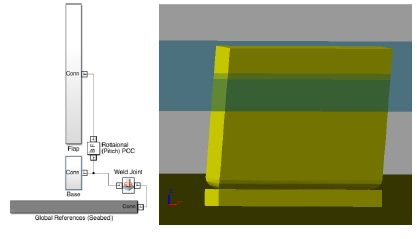
\includegraphics[width=0.99\textwidth]{application/images/OSWEC_WECSim_GUI}
        \caption{OSWEC modeled in WEC-Sim (left-hand side) and with the GUI (right-hand side)}
        \label{OSWEC_WECSim_GUI}
        \end{figure}

%%%%%%%%%%%%%%%%%%%%%%%%%%%%%%%%%%%%%%%%%%%%%%%%%%%%%%%%%%
\section{WEC-Sim Test Cases}
Provided within the applications folder in the WEC-Sim directory are the two applications of the WEC-Sim code. The first application uses the WEC-Sim code to model the the RM3 WEC, and the second application uses the code to model the OSWEC device. Should the WEC-Sim user make changes to the WEC-Sim code, scripts are provided that compare the previous version of WEC-Sim to the latest run, for debugging purposes.  These test cases can be used by running the \texttt{RunTestCase.m} script.  This script imports the \texttt{*.mat} file that contains results from the original WEC-Sim run, and then plots a comparison of the original run to the latest run of WEC-Sim.  

%%%%%%%%%%%%%%%%%%%%%%%%%%%%%%%%%%%%%%%%%%%%%%%%%%%%%%%%%%
\subsection{RM3 Test Case}
For the RM3, the test case is set up for direct comparison using the following model parameters:

\textbf{Wave Environment}   \\
\indent	Wave Type                            = Regular Waves (Sinusoidal Steady-State) \\
	Wave Height H                    (m) = 2.5 \\ 
	Wave Period T                  (sec) = 8 \\

\textbf{WEC-Sim Simulation Settings} \\ 
	Time Marching Solver                 = Fourth-Order Runge-Kutta Formula \\ 
	Start Time                     (sec) = 0  \\
	End Time                       (sec) = 400  \\
	Time Step Size                 (sec) = 0.1 \\
	Ramp Function Time             (sec) = 100 \\

\textbf{List of PTO(s)} \\
	Number of PTOs = 1 \\
	PTO Stiffness           (N/m) = 0 \\
	PTO Damping           (Ns/m) = 1.2E+06 \\

        \begin{figure}[H]
        \centering
        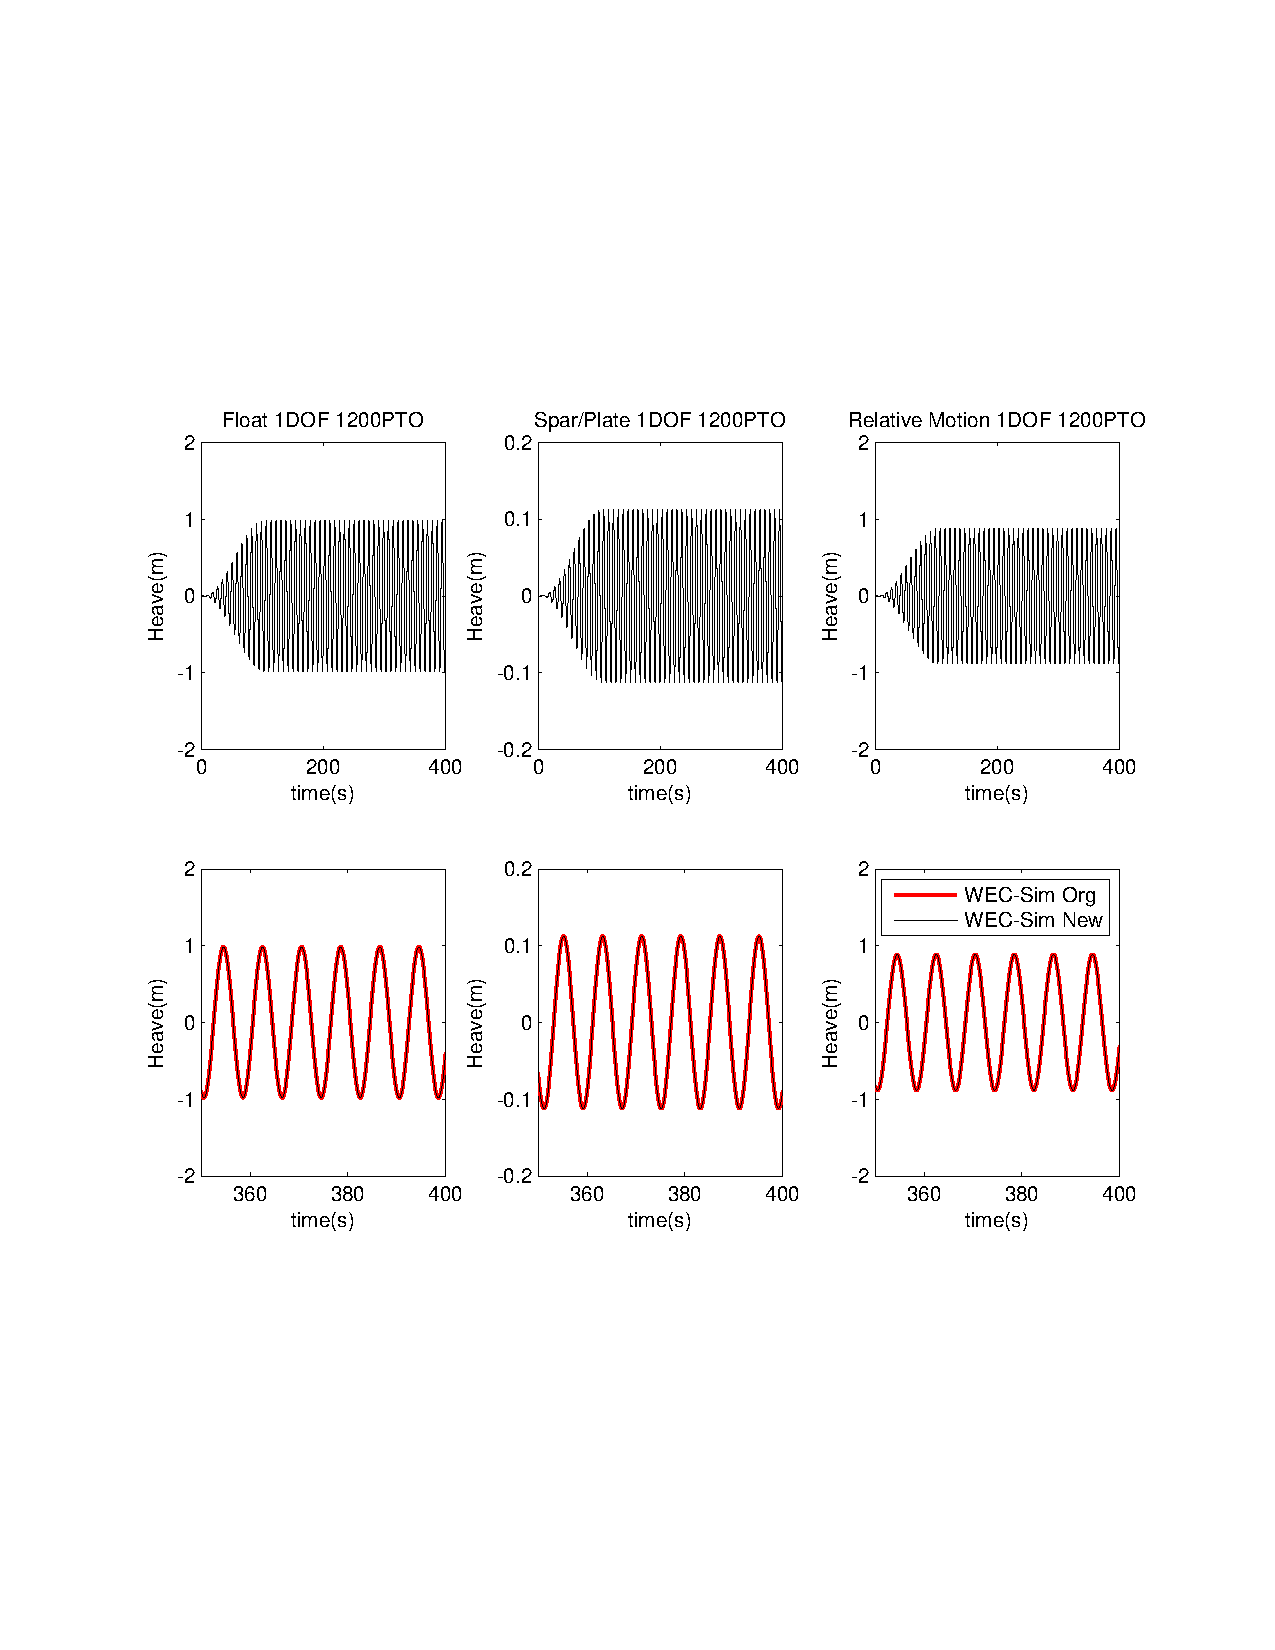
\includegraphics[width=0.99\textwidth]{application/images/RM3_Test}
        \caption{WEC-Sim test plot for RM3: Full simulation (top); last six periods (bottom)}
        \label{RM3_Test}
        \end{figure}

\clearpage

%%%%%%%%%%%%%%%%%%%%%%%%%%%%%%%%%%%%%%%%%%%%%%%%%%%%%%%%%%
\subsection{OSWEC Test Case}
For the OSWEC, the test case is set up for direct comparison using the following model parameters:

\textbf{Wave Environment}   \\
\indent	Wave Type                            = Regular Waves (Sinusoidal Steady-State) \\
	Wave Height H                    (m) = 2.5 \\ 
	Wave Period T                  (sec) = 8 \\

\textbf{WEC-Sim Simulation Settings} \\ 
	Time Marching Solver                 = Fourth-Order Runge-Kutta Formula \\ 
	Start Time                     (sec) = 0  \\
	End Time                       (sec) = 400  \\
	Time Step Size                 (sec) = 0.1 \\
	Ramp Function Time             (sec) = 100 \\

\textbf{List of PTO(s)} \\
	Number of PTOs = 1 \\
	PTO Stiffness           (Nm/rad) = 0 \\
	PTO Damping           (Nsm/rad) = 0 \\

        \begin{figure}[H]
        \centering
        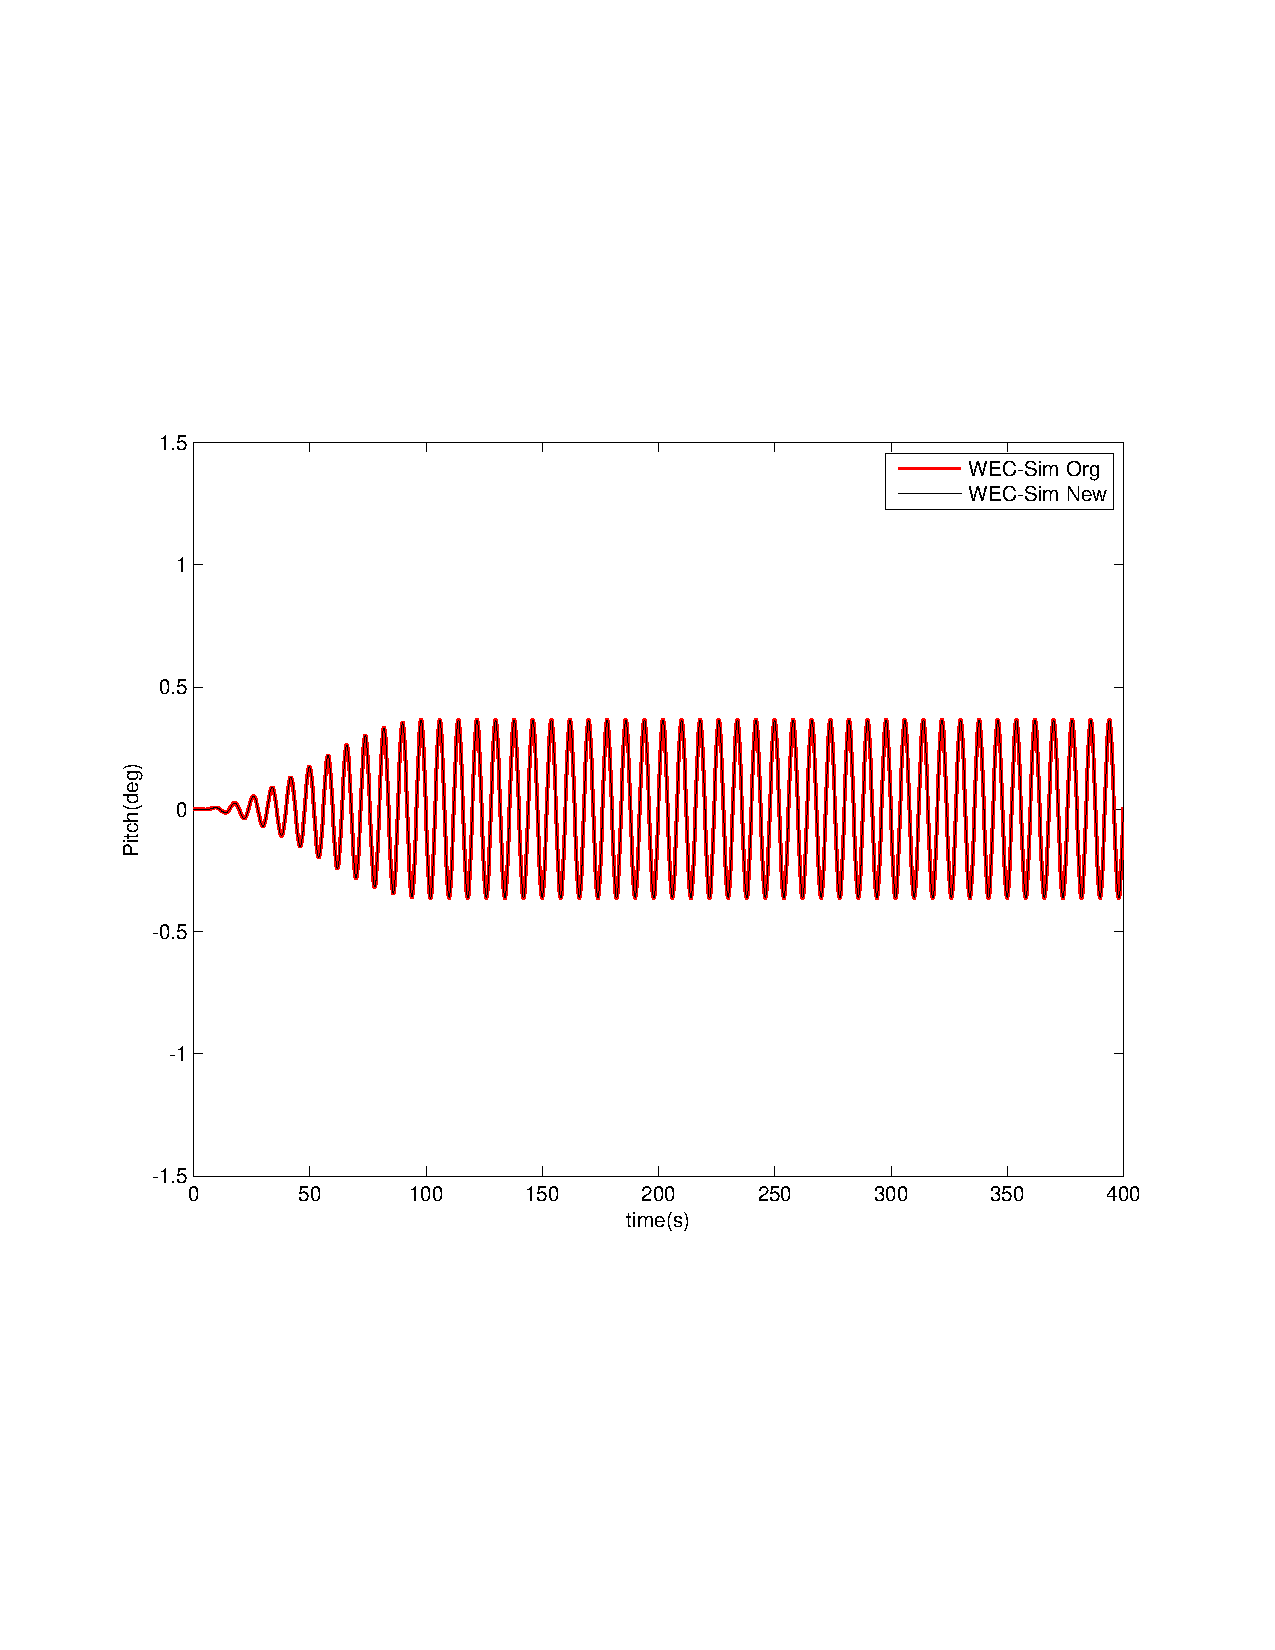
\includegraphics[width=0.55\textwidth]{application/images/OSWEC_Test}
        \caption{WEC-Sim test plot for OSWEC full simulation}
        \label{OSWEC_Test}
        \end{figure}

\clearpage
